\section{Umsetzung in Code}
Im Folgenden werde ich auf die Implementierung der einzelnen Module eingehen und die Besonderheiten, Erfahrungen und Probleme während der Programmierung beschreiben. Um die PDF Web App auch offline nutzen zu können, habe ich die Library-Dateien im Ordner libs direkt eingebunden, anstatt \gls{cdn}-Links zu den jeweiligen Libraries zu verknüpfen. Zur Positionierung von HTML-Elementen habe ich hauptsächlich auf das CSS Flexible Box (Flex Box) Layout zurückgegriffen. 

\subsection{Werkzeuge}
\begin{itemize}
	\item Entwicklungsumgebung: Visual Studio Code
	\item ausführende Programme: Firefox Browser
	\item Sprachen: JavaScript, CSS, HTML
	\item Libraries: Vue JS 3 Version 3.0.2, PDF-LIB, Fontkit zur Einbettung von benutzerdefinierten Fonts, pdf.js, zip,js, Bootstrap Filestyle Version 2.1.0, Bootstrap Version 4.3.1, jQuery Version 3.6.0 dependency von Filestyle, Alwan für den Color Picker
	\item Tutorials: Tiddly Wiki
\end{itemize}

\subsection{Links der Resources}
\begin{itemize}
	\item \url{https://vuejs.org/}
	\item \url{https://pdf-lib.js.org/}
	\item \url{https://www.npmjs.com/package/@pdf-lib/fontkit}
	\item \url{https://github.com/mozilla/pdf.js}
	\item \url{https://github.com/gildas-lormeau/zip.js/}
	\item \url{https://github.com/markusslima/bootstrap-filestyle}
	\item \url{https://getbootstrap.com/}
	\item \url{https://jquery.com/}
	\item \url{https://github.com/SofianChouaib/alwan}
	\item \url{https://tiddlywiki.com/}
\end{itemize}

\subsection{Ordnerstruktur}
Abbildung \ref{fig:folders} stellt die Ordnerstruktur des Projekts dar. 

\begin{figure}[!htbp]
	\centering
	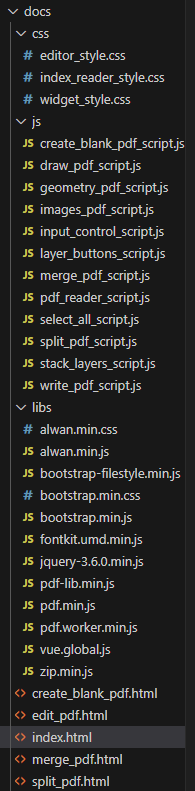
\includegraphics[width=0.3\textwidth]{"images/folders.png"}
	\caption{Ordnerstruktur der PDF Web App}
	\label{fig:folders}
\end{figure}

In den Ordnern js sind meine selbst geschriebenen JavaScript- und in css meine eigenen CSS-Dateien abgelegt. Genauso wurden alle HTML-Dateien von mir erstellt. Der Ordner libs enthält alle JavaScript- und CSS-Dateien von externen Libraries. Die Datei pdf.worker.min.js ist eine dependency von pdf.js und fontkit.umd.min.js gehört zur Library PDF-LIB, um benutzerdefinierte Fonts einzubinden. Im Prinzip hat jedes Modul seine eigene JavaScript-Datei. Das Script input\_control\_script.js, welches global implementiert wird, enthält Kontrollfunktionen für Benutzereingabefelder (Input Control) und die ZIP-Download-Funktionen. Der Editor teilt sich die Dateien pdf\_reader\_script.js und index\_reader\_style.css mit dem Reader. Die CSS-Datei widget\_style.css deckt den Creator, Merger und Splitter ab. Der Editor besteht aus mehreren Scripten: write\_pdf\_script.js für Text, draw\_pdf\_script.js für Drawings, geometry\_pdf\_script.js für Shapes, images\_pdf\_script.js für Images, layer\_buttons\_script.js für das Layers Menu, select\_all\_script.js für die Selection and Deselection Filter Menus und stack\_layers\_script.js für Layers-Managementfunktionen. Reader, Splitter und Merger besitzen jeweils eine separaten HTML-Seite. Das Editormodul ist eine einzelne HTML-Seite, bei der je nach Funktion die entsprechenden Schaltflächen für die Elementoperationen mit display: flex eingeblendet und display: none ausgeblendet werden. 

\subsection{Layoutgestaltung}
Das Hauptmenü wollte ich minimalistisch, klar und übersichtlich gestalten. Daher habe ich für die Startseite lediglich einen weißen Hintergrund gewählt mit einem oberen Balken in der Farbe \#333 als dunkles Grau zur Hervorhebung der Hauptmenübuttons. Dasselbe dunkle Grau wiederholt sich in den beiden oberen Reader-Leisten und dem Reader-Hintergrund. Die Buttons haben einen vordefinierten Style von der Library Bootstrap. In der Bootstrap-Library kann der Style durch fixe Klassen bestimmt werden. Alle grünen Buttons und die selection menus im Creator und Splitter haben die Bootstrap-Klasse btn-success. Der dunkelgraue Button mit grüner Schrift und Umrandung des aktiven Hauptmenü-Buttons besitzt die Bootstrap-Klasse btn-outline-success. Die Beschriftung des Buttons für Choose file (INPUT type file HTML-Element) ist standardmäßig in Deutsch gehalten und lässt sich grundsätzlich nicht in englischer Sprache programmieren. Aus diesem Grund habe ich die Library Bootstrap Filestyle verwendet, um den Choose file-Button in Englisch zu beschriften. Um eine Designkonsistenz zu erzielen, habe ich die Bootstrap-Buttons flächendeckend in der GUI in verschiedenen Stylevarianten verwendet. Lediglich bei Tools im Editor habe ich einen eigenen Style für die Buttons der Elementoperationen programmiert. Diese weißen Buttons besitzen eine schwarze Schrift mit einer border-width von 2 Pixeln, einem border-radius von 5 Pixeln und einer border-color von \#333. Der inaktive, weiße Modus-Button und die ausgeschalteten Selection und Deselection Filter in Layers sind mit dem Bootstrap-Style btn-light versehen. Alle dunkelgrauen Buttons wurden mit dem Bootstrap-Style btn-dark implementiert. Jegliche rosa Flächen und ausgewählte Layers haben die Farbe \#dabdb6. Der hellgraue Operations Bar und das Namensfeld einer Layer sind in \#8c8c8c (Hellgrau) gefärbt. Tools und aktivierte checkboxes haben eine Hintergrundfarbe in \#5eb873 (Türkis). Der Hintergrund von Layers, Layers Menu, sowie die Seitengruppen und Tools besitzen einen Alphawert von 0.8. Abgewählte Layers, selection menus in Tools, der Hintergrund beim Output-Dateinamen und ausgewählte Dateinamen im Merger sind schwarz. Alle Horizontal-Leisten mit Operationen haben eine Höhe von 58 Pixeln und dessen Buttons einen horizontalen Abstand von 5 Pixeln. Layers und Tools sind jeweils 190 Pixel breit. In Dateinamen von Font- und Bilddateien wird nach 15 Zeichen ein Zeilenumbruch eingefügt. Der Dateiname des Output-PDFs ist auf 50 Zeichen beschränkt. Im Reader befinden sich zwischen den gerenderten Seiten 20 Pixel Abstand. Alle input fields, Scrollbars und INPUT type checkbox HTML-Elemente besitzen den default Style des Browsers. Die default Dateinamen für Reader und Editor sind wie folgt benannt: Source-Dokument Dateiname, ein Unterstrich und edited. Der Creator benennt standardmäßig die Output-Datei mit blank\_pdf und der Merger mit merged\_pdf. Im Splitter wird als Dateibenennungsschema der source-Dateiname, ein Unterstrich und split verwendet. 

\subsection{Input Control}
Eine automatisierte Eingabekontrolle von Benutzereingabefeldern findet in allen Modulen außer dem Merger statt. Alle input fields sind INPUT type text HTML-Elemente, anstatt type number – selbst wenn nur Zahlen als Eingabewerte gültig sind. Das hat folgenden Hintergrund: Es gibt eine Funktion restrictInputValues, die automatisch Benutzereingaben korrigiert. Die Funktion wird ausgelöst, sobald das input field verändert wurde (change event). Im Prozess wird der event handler zunächst entfernt, bevor er angeheftet wird. Würde der event handler nicht initial abgekoppelt werden, würde dieses Eingabefeld immer mehr event handler akkumulieren. RestrictInputValues entfernt jeglichen white space, wandelt die Benutzereingaben als String in Zahlen um und hält die eingegebenen Werte in einem gültigen Wertebereich. Außerdem habe ich eine Funktion convertInputToSuccess programmiert, die den Input-String in einen Zahlenwert parst und den geparsten Wert oder -1000 (invalid input) zurückgibt. Die return value von convertInputToSuccess bestimmt maßgeblich, ob Operationen, z.B. die Font Size im Writer, ausgeführt werden sollen. Für die Eingabe einer Seitenliste, existiert eine gesonderte Funktion convertPagelistToSuccess. An dieser Stelle wird bei invalid input die Benutzereingabe zurückgesetzt. Eine genauere Beschreibung des Verhaltens der Input Control werde ich im Unterkapitel Testdurchführung, Abschnitt Testauswertung, weiter ausführen.

\subsection{Einlesen einer PDF-Datei im Reader und Editor}
Die Funktion für den Choose file-Button ist in Codeabschnitt \ref{code:file} dargestellt.

\begin{lstlisting}[style=ES6, caption={Einlesen einer PDF-Datei}, label=code:file, breaklines=true]
	let inputFileButtons = document.getElementsByClassName('inputfile');
	for (let i = 0; i < inputFileButtons.length; i++) {
		inputFileButtons[i].addEventListener("change", function(e) {
			resetAllModes();
			// ...
			file = e.target.files[0];
			const fileReader = new FileReader(); 
			fileReader.onload = function() {
				const typedarray = new Uint8Array(this.result);
				const pdfBytes = typedarray;
				const loadingTask = pdfjsLib.getDocument(typedarray);
				loadingTask.promise.then(async (pdf) => {
					if (file.name.endsWith(".pdf")) {
						try {
							outputPDF = await PDFLib.PDFDocument.load(pdfBytes);
						} catch(encryptedErr) {
							encrypted = true;
						}
						if (!encrypted) {
							if (pdf._pdfInfo.numPages <= 5000) {
								pdfState.pdf = pdf;
								pdfState.originalPDFBytes = pdfBytes;
								pdfState.existingPDFBytes = pdfBytes;
								// ...
								pdfState.lastPage = pdf._pdfInfo.numPages;
								// ...
								adjustPDFToUserViewport();
								pdfState.renderedPage = 0;
								// ...
								let readerMode = true;
								let editorMode = false;
								const openPDFs = document.getElementsByClassName("open_pdf");
								for (let i = 0; i < openPDFs.length; i++) {
									if (openPDFs[i].classList.contains("btn-outline-success")) {
										readerMode = true;
										break;
									} else if (openPDFs[i].classList.contains("btn-success")) {
										readerMode = false;
									}
								}
								const editorBtns = document.getElementsByClassName("editor_btn");
								for (let i = 0; i < editorBtns.length; i++) {
									if (editorBtns[i].classList.contains("btn-outline-success")) {
										editorMode = true;
										break;
									} else if (editorBtns[i].classList.contains("btn-success")) {
										editorMode = false;
									}
								}
								if (!readerMode && editorMode) {
									onetimeSetup = true;
									// ...
									setTimeout(initEditor, 300);
								}
								startRender = performance.now();
								await renderPage(pageCounter, false);
							} else {
								pagesError = true;
								for (let i = 0; i < pagesErrorWidgets.length; i++) {
									pagesErrorWidgets[i].style.display = "flex";
								}
							}
						} else {
							encryptedError = true;
							for (let i = 0; i < encryptedErrorWidgets.length; i++) {
								encryptedErrorWidgets[i].style.display = "flex";
							}
						}
					}
				}).catch(unsupportedFileErr => {
					noPDFError = true;
					for (let i = 0; i < noPDFErrorWidgets.length; i++) {
						noPDFErrorWidgets[i].style.display = "flex";
					}
				});
			}
			if (file) {
				fileLoaded = true;
				fileReader.readAsArrayBuffer(file);
			}
		}, false);
	}
\end{lstlisting} 

Bei jedem Klick auf den Choose File-Button werden alle Modi für aktive Operation-Buttons des Editors und andere Steuerungsmodi in der Funktion resetAllModes auf false gesetzt. Die Datei wird mittels eines FileReader-Objekts eingelesen und dem load event wird eine anonyme Funktion zugewiesen. Die eingelesene PDF-Datei, bestehend aus einem Uint8Array, wird in den properties originalPDFBytes und existingPDFBytes des globalen Objekts pdfState gespeichert. Die PDF-LIB-Funktion für das Laden eines PDFs akzeptiert einen Parameter vom Typ Uint8Array. Die PDF-LIB-Speicherfunktion gibt ein als Uint8Array serialisiertes PDF zurück. Im Editor wird bei jedem Downloadvorgang des modifizierten PDFs das originale PDF als Grundlage zur Einbettung verwendet (originalPDFBytes). Das Objekt pdfState, welches den aktuellen Anzeige- und Datenstatus des eingelesenen PDFs repräsentiert, ist in einem Codeschnipsel \ref{code:pdfstate} dargestellt:

\begin{lstlisting}[style=ES6, caption={Objekt für den Status eines geöffnetes PDF-Dokuments}, label=code:pdfstate, breaklines=true]
	let pdfState = {
		pdf: null,
		currentPage: 1,
		lastPage: 1,
		renderedPage: 0,
		zoom: 1,
		originalPDFBytes: null,
		existingPDFBytes: null,
		originalWidths: [],
		originalHeights: []
	}
\end{lstlisting} 

Eine loadingTask wird durch die pdf.js-Funktion getDocument erzeugt, die ein libraryinternes pdf-Objekt zurückliefert. Dieser Return-Wert wird in pdfState.pdf abgelegt. In pdfState.lastPage wird die Seitenzahl der letzten Seite gespeichert. Das pdf.js-eigene pdf-Objekt wird für das Rendern der PDF-Seiten im Reader und Editor benötigt. Weiter in der anonymen Funktion wird das PDF dem Viewport des Browsers mit einem horizontalen Abstand von 100 Pixeln pro Fensterseite angepasst. Anschließend wird pdfState.renderedPage initialisiert. Dieses property enthält die aktuell gerenderte Seite, die am Ende des Rendervorgangs der letzten Seite des PDFs entspricht. Ob es sich um den Reader oder Editor handelt, wird überprüft, indem die Bootstrap-Klassen der zugehörigen Hauptmenü-Buttons abgefragt werden. Falls der Editor geöffnet wurde, wird er mit einer Zeitverzögerung von 300 ms aufgebaut. Hintergrund dessen ist, dass die vorherige \gls{dom}-Version erst gerendert werden muss, sonst ergibt sich bei Zugriff auf HTML-Collections – ein arrayähnliches Objekt – eine Length von 0. Am Ende wird der Rendervorgang durch die rekursive, asynchrone Funktion renderPage in Gang gesetzt. Das \gls{dom} ist eine Web API für Webdokumente wie HTML-Dokumente. Es repräsentiert die Webseite als nodes und Objekte, sodass Programmiersprachen die Dokumentenstruktur, -style und -inhalt modulieren können. Strukturell besteht das \gls{dom} aus dem \gls{dom} tree, dessen nodes den HTML-Inhalt repräsentieren. Im \gls{dom} sind alle properties, Methoden und events für die Manipulation und Erzeugung von Webseiten als Objekte organisiert \cite{mozilla-dom}. 

\subsection{Renderfunktion}
Im Codeauszug \ref{code:render} ist die Funktion renderPage abgebildet.

\begin{lstlisting}[style=ES6, caption={Renderfunktion}, label=code:render, breaklines=true]
	async function renderPage(num, renderSingle) {
		pdfState.pdf.getPage(num).then(function(page) {
			let viewport = page.getViewport({
				scale: pdfState.zoom
			});
			let viewportOriginal = page.getViewport({
				scale: 1
			});
			let canvas;
			let div;
			const pdfViewers = document.getElementsByClassName("pdf_viewer");
			for (let i = 0; i < pdfViewers.length; i++) {
				const pdfViewer = pdfViewers[i];
				// ...
				if (writeLayerStack.length < pdfState.pdf._pdfInfo.numPages) {
					div = document.createElement("div");
					div.style.display = "flex";
					div.width = viewport.width;
					div.height = viewport.height;
					div.style.width = viewport.width + "px";
					div.style.height = viewport.height + "px";
					div.style.marginBottom = "20px";
					pdfState.originalWidths.push(viewportOriginal.width);
					pdfState.originalHeights.push(viewportOriginal.height);
					div.setAttribute('data-write', pageCounter);
					div.classList.add("write_layer");
					canvas = document.createElement("canvas");
					canvas.style.display = "flex";
					canvas.width = viewport.width;
					canvas.height = viewport.height;
					canvas.style.width = viewport.width + "px";
					canvas.style.height = viewport.height + "px";
					canvas.setAttribute('data-page', pageCounter);
					canvas.classList.add("render_context");
					div.appendChild(canvas);
					pdfViewer.appendChild(div);
					writeLayerStack.push(div);
				} else if (writeLayerStack.length === pdfState.pdf._pdfInfo.numPages) {
					if (!renderSingle) {
						div = writeLayerStack[pageCounter-1];
						canvas = writeLayerStack[pageCounter-1].childNodes[0];
					} else {
						div = writeLayerStack[num-1];
						canvas = writeLayerStack[num-1].childNodes[0];
					}
					div.width = viewport.width;
					div.height = viewport.height;
					div.style.width = viewport.width + "px";
					div.style.height = viewport.height + "px";
					canvas.width = viewport.width;
					canvas.height = viewport.height;
					canvas.style.width = viewport.width + "px";
					canvas.style.height = viewport.height + "px";
				}
			}
			const context = canvas.getContext('2d');
			let renderTask = page.render({
				canvasContext: context,
				viewport: viewport
			});
			if (!renderSingle) {
				renderTask.promise.then(function() {
					pdfState.renderedPage = pageCounter;
					// ...
					pageCounter++;
					// ...
					if (pdfState.pdf != null && pageCounter <= pdfState.pdf._pdfInfo.numPages) {
						renderPage(pageCounter, false);
					}
				});
			}
		});
	}
\end{lstlisting} 

Die Funktion ruft sich für alle noch nicht gerenderten Seiten rekursiv auf. Sie kann den Rendervorgang für eine oder alle Seiten vornehmen. Eine einzelne Seite wird neu gerendert, sobald sie im Reader gedreht wurde. Pro Funktionsaufruf wird der globale pageCounter hochgezählt. Mittels des pdfState.pdf-Objekts wird die aktuelle Seite geholt und ein Seitenobjekt von pdf.js entgegengenommen. Aus diesem Seitenobjekt wird der Viewport der Seite extrahiert und eine Skalierung festgelegt. PdfState.zoom, welches die aktuelle Skalierung des gesamten PDF-Dokuments angibt, wird der Viewport-Skalierung zugewiesen. Viewport besitzt width und height properties. Zusätzlich wird der Viewport mit einer Skalierung von 1 gespeichert. Hintergrund dessen ist, dass im weiteren Verlauf von renderPage die Arrays pdfState.originalWidths und pdfState.originalHeights die Originalgrößen jeder Seite aufnehmen sollen. Der Container des gerenderten PDFs besteht aus mehreren verschachtelten DIV-HTML-Elementen, wobei das innere Element die Klasse pdf\_viewer besitzt. Dem inneren pdf\_viewer-Container werden pro Ausführung von renderPage ein DIV mit der Klasse write\_layer und ein Attribut data-write, was die zugehörige Seitenzahl speichert, hinzugefügt. Die write\_layer symbolisiert einen Seitencontainer, der die gerenderte PDF-Seite und beigefügten Elemente des Editors enthält. Die gerenderte PDF-Seite wird in einem CANVAS-HTML-Element als erstes child der write\_layer dargestellt. Diese CANVAS hat die Klasse render\_context und ein Attribut data-page für die identische Seitenzahl der write\_layer. Sowohl die write\_layer als auch der render\_context werden in der Größe des aktuell skalierten Viewports angelegt. Die write\_layers werden zusätzlich in einem Array writeLayerStack gesammelt. WriteLayerStack hält die write\_layers in der Reihenfolge der PDF-Seiten im Dokument. Während eines erneuten Rendervorgangs wird der render\_context wiederverwendet. Anschließend wird mittels der pdf.js-Library die Seite gerendert. Nach Beendigung der renderTask wird eine anonyme Funktion ausgeführt. Die pageCounter-Variable wird pdfState.renderedPage zugewiesen. Dieses property wird als Maximalwert für die Input Control bei der Navigation zu einer bestimmten Seite verwendet.

\subsection{Implementierung der Vue JS 3-Module}
Die Module Creator, Splitter und Merger verwenden das Framework Vue JS 3, zwar nicht in nativer Form als \gls{spa}, sondern als stand-alone widgets. Im Creator wird annähernd die eingestellte PDF-Seitengröße als Breite und Höhe der MediaBox durch die Berechnung in den Codezeilen \ref{code:mediabox} gesetzt. Diese Berechnung habe ich durch Tests erarbeitet.

\begin{lstlisting}[style=ES6, caption={Berechnung der PDF-Seitengröße}, label=code:mediabox, breaklines=true]
const pageWFactor = (blankPageWidth * 1000) / 352.8;
const pageHFactor = (blankPageHeight * 1000) / 352.8;
for (let i = 0; i < blankNumOfPagesCount; i++) {
	page = pdfDoc.addPage();
	page.setMediaBox(0, 0, pageWFactor, pageHFactor);
}
\end{lstlisting} 

Durch Anwählen der Portrait-Orientierung wird in den Width and Height input fields der kleinere Wert der Seitendimensionen für die Width gesetzt und der größere Wert für die Height. Im Falle von Landscape werden Width und Height vertauscht. Quadratic orientiert sich an der Width.
\par
Nach Aufruf des Splitters wird zunächst ein gesperrter Save-Button vorgefunden. Die Benutzbarkeit des Save-Buttons wird erst freigeschaltet, nachdem eine Datei und Split-Methode im selection menu ausgewählt wurde. Unter dem Choose file-Button ist der auf 50 Zeichen gekürzte Dateiname abgebildet. Erst wenn list of pages selektiert wurde, wird das input field für die Seitenliste aktiviert. Die Split-Funktion für gerade und ungerade Seiten nennt sich SplitAfter. Basierend auf den Rest Modulo 2 wird die Funktion mit der Bedingung ausgeführt, dass bei der even pages-Split-Methode mehr als 3 Seiten bzw. bei der odd pages-Split-Methode mehr als 2 Seiten im Input-PDF vorhanden sind. Andernfalls bleibt der Save-Button deaktiviert. Die Input-PDF Bestandteile als Dokumentobjekte von PDF-LIB, die nach jedem Split-Vorgang bei der PDF-LIB-Funktion PDFDocument.create entstehen, werden in einem globalen Array splittedPDFs gesichert. Die Arraybestandteile werden einzeln durch Klick auf Save zu einem Uint8Array serialisiert und in einem globalen Array pdfBytesList gespeichert. PdfBytesList wird letztendlich der compressMultipleToZip-Funktion übergeben. Jedes gesplittete PDF erhält den Ursprungsdateinamen, einen Unterstrich und einen Index beginnend mit 0, der das Teil-PDF aufsteigend in der Split-Reihenfolge nummeriert. Alle PDF-Bestandteile werden als ZIP-Ordner verpackt. Am Ende des Downloads werden splittedPDFs und pdfBytesList als leere Arrays initialisiert.
\par
Im Merger wird eine geöffnete Datei als Uint8Array einem globalen Array selectedPDFBytes hinzugefügt. Zusätzlich wird einem UL-HTML-Element, dem Dateilistencontainer, pro Datei ein LI-HTML-Element mit der Klasse file\_unselected angehängt. Außerdem wird der auf 50 Zeichen gekürzte Dateinamen und ein click event handler für die Dateimarkierung hinzugefügt. Sind mehr als eine oder maximal 100 Dateien ausgewählt, schalten sich Save und Remove ein. Außerdem wird der LI eine Reihe an drag events hinzugefügt: Dragstart, dragover und drop. Funktion der drag events ist, dass die Listeneinträge in ihrer Reihenfolge alterniert werden können. Zu jedem Zeitpunkt spiegelt das Array selectedPDFBytes die Reihenfolge der Listeneinträge wieder. Für das dragging muss der Listeneintrag nicht markiert sein, jedoch beim Entfernen von einzelnen Listeneinträgen. Ist ein Listeneintrag schwarz markiert, wird die Klasse file\_unselected mit der Klasse file\_selected des entsprechenden LI ersetzt.

\subsection{Struktur der Editorelemente}
Die 4 Editorelemente Text, Drawing, Shape und Image werden bei Erzeugung auf der Seite in globalen Arrays als Elementlisten in Erstellungsreihenfolge abgelegt: userTextList für Text, drawLayerStack für Drawings, geometryPointsList für Shapes und userImageList für Images. Zur Erstellung der Editorelemente verwende ich zum einen Objekte, welche die Nodestruktur der Elemente in der Webseite abbilden. Zum anderen setze ich Objekte ein, die die elementspezifischen Eigenschaften repräsentieren. Genannte Objekte erben von Prototyp-Objekten gemäß dem Konzept der prototypischen Objektorientierung. Im Codeabschnitt \ref{code:control-point} ist das strukturelle Prototyp-Objekt für Text, Drawing und Image abgebildet. Der darauffolgende Codeabschnitt \ref{code:shape-controller-point} zeigt das strukturelle Prototyp-Objekt für Shape.

\begin{lstlisting}[style=ES6, caption={Prototyp-Objekt für die Node-Struktur von Text, Drawing und Image}, label=code:control-point, breaklines=true]
	let controlPoint = {
		controlBox: null,
		editImg: null,
		elementToControl: null,
		type: '',
		layer: null,
		page: 1,
		x: 0,
		y: 0,
		index: 0,
		setControlPoint() {
			let div = document.createElement("div");
			div.style.position = "absolute";
			div.style.left = this.x + "px";
			div.style.top = this.y + "px";
			div.setAttribute('data-page', this.layer.getAttribute("data-write"));
			div.setAttribute('data-index', this.index);
			div.classList.add(this.type);
			div.classList.add("box");
			this.controlBox = div;
		}
	}
\end{lstlisting}

\begin{lstlisting}[style=ES6, caption={Prototyp-Objekt für die Node-Struktur von Shape}, label=code:shape-controller-point, breaklines=true]
	let shapeControllerPoint = {
		controlBox: null,
		editImg: null,
		elementToControl: null,
		layer: null,
		page: 1, 
		x: 0,
		y: 0,
		index: 0, 
		rotation: 0,
		originX: 0,
		originY: 0,
		setControlPoint() {
			let div = document.createElement("div");
			div.style.position = "absolute";
			div.style.left = this.x + "px";
			div.style.top = this.y + "px";
			div.setAttribute('data-page', this.layer.getAttribute("data-write"));
			div.setAttribute('data-index', this.index);
			div.classList.add("shape");
			div.classList.add("box");
			this.controlBox = div;
		},
		rotateControlPoint() {
			this.controlBox.style.marginLeft = this.originX + "px";
			this.controlBox.style.marginTop = this.originY + "px";
			this.controlBox.style.transform = "rotate(" + this.rotation + "deg)";
		}
	}
\end{lstlisting}  

Vom controlPoint-Prototyp leitet das Objekt controlP ab und von shapeControllerPoint erbt shapeControllerP. ShapeControllerPoint stellt einen spezialisierten controlPoint dar, der mit Rotations-properties und einer Rotations-Methode erweitert wurde. ControlP- und shapeControllerP-Objekte werden direkt in userTextList, drawLayerStack, userImageList und geometryPointsList gespeichert. Die Prototypen besitzen ein property elementToControl, um die Objekte mit elementspezifischen Eigenschaften zu referenzieren. Dessen Prototypen heißen userText für Text, drawLayer für Drawings, shape für Shapes und userImage für Images. Sie sind in den Codesegmenten \ref{code:user-text}, \ref{code;draw-layer}, \ref{code:shaoe} und \ref{code:user-image} aufgeführt.

\begin{lstlisting}[style=ES6, caption={Prototyp-Objekt für die textspezifischen Eigenschaften}, label=code:user-text, breaklines=true]
	let userText = {
		pdfDoc: null,
		pdfBytes: null,
		text: '',
		x: 1,
		y: 1,
		size: 1,
		fontKey: null,
		font: null,
		lineHeight: 34,
		color: rgb(0, 0, 0),
		page: 1,
		opacity: 1.0,
		rotation: degrees(0),
		setTextElem() {
			this.pdfDoc.getPages()[0].drawText(this.text, {
				x: this.x,
				y: this.y,
				size: this.size,
				font: this.font,
				color: this.color,
				lineHeight: this.lineHeight,
				rotate: this.rotation
			});
		}
	}
\end{lstlisting}

\begin{lstlisting}[style=ES6, caption={Prototyp-Objekt für die drawingspezifischen Eigenschaften}, label=code:draw-layer, breaklines=true]
	let drawLayer = {
		paths: [],
		currentPathIndex: 0, 
		rotation: 0,
		wasRotated: false
	}
\end{lstlisting}

\begin{lstlisting}[style=ES6, caption={Prototyp-Objekt für die shapespezifischen Eigenschaften}, label=code:shape, breaklines=true]
	let shape = {
		context: null,
		type: "",
		x: 0,
		y: 0,
		xp2: 50,
		yp2: 50,
		width: 100,
		height: 100,
		stroke: 'rgba(0,0,0,1.0)',
		strokeWidth: 3,
		fill: '',
		useFill: false,
		useStroke: false,
		rotation: 0,
		page: 1,
		drawShape() {
			if(this.type === "rectangle") {
				let rectCenterX = this.x + this.width / 2;
				let rectCenterY = this.y + this.height / 2;
				this.context.save();
				this.context.beginPath();
				this.context.translate(rectCenterX, rectCenterY);
				this.context.rotate(this.rotation * Math.PI / 180);
				this.context.translate(-rectCenterX, -rectCenterY);
				if (this.useFill) 
				this.context.fillStyle = this.fill;
				if (this.useStroke) {
					this.context.strokeStyle = this.stroke;
					this.context.lineWidth   = this.strokeWidth;
				}
				if (this.useFill) {
					this.context.fillRect(this.x, this.y, this.width, this.height);
				}
				if (this.useStroke) {
					this.context.strokeRect(this.x, this.y, this.width, this.height);
				}
				this.context.restore();
			} else if (this.type === "triangle") {
				let triCenterX = this.x + this.width / 2;
				let triCenterY = this.y + this.height / 2;
				this.context.save();
				this.context.beginPath();
				this.context.translate(triCenterX, triCenterY);
				this.context.rotate(this.rotation * Math.PI / 180);
				this.context.translate(-triCenterX, -triCenterY);
				this.context.moveTo(this.x, this.y);
				this.context.lineTo(this.x, this.y + this.height);
				this.context.lineTo(this.x + this.xp2 + this.width, this.y + this.yp2);
				this.context.closePath();
				
				if (this.useFill) 
				this.context.fillStyle = this.fill;
				
				if (this.useStroke) {
					this.context.strokeStyle = this.stroke;
					this.context.lineWidth   = this.strokeWidth;
				}
				
				if (this.useFill) 
				this.context.fill();
				
				if (this.useStroke)    
				this.context.stroke();
				
				this.context.restore();
			} else if (this.type === "circle") {
				this.context.beginPath();
				this.context.ellipse(this.x, this.y, this.width / 2, this.height / 2, this.rotation * Math.PI / 180, 0, 2 * Math.PI);
				
				if (this.useFill) {
					this.context.fillStyle = this.fill;
				}
				if (this.useStroke) {
					this.context.strokeStyle = this.stroke;
					this.context.lineWidth   = this.strokeWidth;
				}   
				this.context.closePath();
				if (this.useFill) {
					this.context.fill();
				}
				if (this.useStroke)    
				this.context.stroke();
			}
		}
	}
\end{lstlisting}

\begin{lstlisting}[style=ES6, caption={Prototyp-Objekt für die imagespezifischen Eigenschaften}, label=code:user-image, breaklines=true]
	let userImage = {
		pdfDoc: null,
		pdfBytes: null,
		image: null,
		base64String: "",
		type: "",
		x: 1,
		y: 1,
		width: 1,
		height: 1,
		page: 1,
		opacity: 1.0,
		rotation: degrees(0),
		setImageElem() {
			this.pdfDoc.getPages()[0].drawImage(this.image, {
				x: this.x,
				y: this.y,
				width: this.width,
				height: this.height,
				rotate: this.rotation,
			});
		}
	}
\end{lstlisting}

Die spezifischen Objekte zu ihren Prototypen nennen sich currentUserText für userText, drawingLayer für drawLayer, currentShape für shape und currentUserImage für userImage. Sowohl die Nodestrukturobjekte als auch die Eigenschaftsobjekte werden durch Hinzufügen von Elementen auf der Seite erstellt und mit Standardwerten initialisiert. 

\subsection{Aufbau eines PDF-Seitencontainers}
Die Wurzel eines PDF-Seitencontainers bildet ein DIV mit der Klasse write\_layer. Write\_layer hat mindestens ein child und eine CANVAS mit der Klasse render\_context. Dieser Fall liegt vor, wenn noch keine Elemente der Seite hinzugefügt wurden. Der render\_context lässt sich als Zeichenfläche vorstellen, die durch die Dimensionen der Seite begrenzt ist. Er enthält die gerenderte Seite als Hintergrund für Elementoperationen. Sobald Elemente auf der Seite ergänzt wurden, stapeln sich weitere Schichten auf dem render\_context. Ein Editorelement setzt sich zusammen, aus einer CANVAS (editimg) für die Darstellung und einem 40 x 40 Pixel-großen DIV (controlBox) für den Kontrollpunkt des Elements. Die CANVAS besitzt 3 Klassen: Editimg, visible und eine Elementtyp-Klasse. Die Klasse editimg konkretisiert die CANVAS, die das gerenderte, einzelne Element enthält. Visible definiert den Sichtbarkeitsstatus über die Ebenensteuerung in Layers. Die Typklasse kann entweder text, drawing, shape oder image sein. Jedes editimg enthält zudem ein data-page-Atribut für die Seitenzahl und data-index für die Position in der Elementliste. Die Größe des editimgs entspricht immer der Größe des zugehörigen render\_context. Auf der controlBox habe ich eine Reihe von event handler definiert, die die Operationen im Operations Bar und in Tools ausführen. Sie besitzt eine Typklasse und die Klasse box, um alle controlBoxes im Dokument ansprechen zu können. Die controlBox ist ebenfalls mit den gleichen data-Attributen wie das zugehörige editimg ausgestattet. Bei Erzeugung wird das zuletzt erstellte editimg oberhalb des Stapels positioniert. Alle editimgs werden in einem Gruppierungs-DIV mit der Klasse editimg\_group akkumuliert. Ebenfalls werden alle controlBoxes in einem gruppierenden DIV mit der Klasse control\_group vereint. Die editimg\_group liegt über dem render\_context im Node Tree-Segment. Ganz oben befindet sich die control\_group, damit controlBoxes nicht von gerenderten Elementen verdeckt werden. Die control\_group und editimg\_group werden beim Hinzufügen des ersten Elementes auf der Seite erstellt. Jede write\_layer hat jeweils eine editimg\_group und control\_group. Das Node-Tree Segment für den Aufbau einer write\_layer ist in Screenshot \ref{fig:write-layer} veranschaulicht. 

\begin{figure}[!htbp]
	\centering
	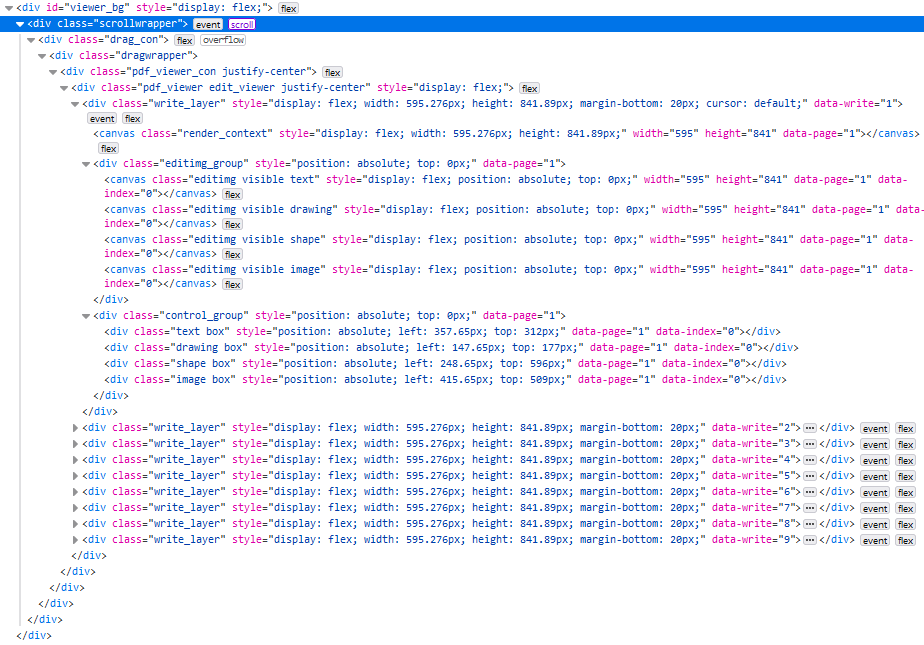
\includegraphics[width=1\textwidth]{"images/write-layer.png"}
	\caption{Node-Tree Segment für den Aufbau einer write\_layer mit 4 Elementen jedes Typs}
	\label{fig:write-layer}
\end{figure}

Für editimg und controlBox existieren gleichnamige properties in den Nodestrukturobjekten. Dort wird die CANVAS und das DIV abgespeichert. Außerdem gibt es ein layer property, in dem die zugehörige write\_layer gesichert ist. In den properties type wird der Elementtyp als String hinterlegt, page beschreibt die Seitenzahl, x und y sind die Koordinaten auf der Seite und index ist die Position des Elements in der zugehörigen Elementliste. Die Reihenfolge der Elemente in userTextList, drawLayerStack, geometryPointsList und userImageList ändert sich nie, es sei denn, ein Element wird von der Seite entfernt. Sowohl der index als auch data-index in den Nodestrukturobjekten müssen immer in editimg und controlBox übereinstimmen. Über diesen maßgeblichen index kann auf das Element in der jeweiligen Elementliste zugegriffen und die zugehörige Layer kann zugeordnet werden.

\subsection{Hinzufügen von Elementen}
Jedes Element hat seine separate Funktion zur Platzierung auf der Seite. Innerhalb dieser Funktion wird createStackLayer aufgerufen, um eine Layer mit dem Element zu verknüpfen. Am Ende des Funktionsbodies der Platzierungsoperation wird das Nodestrukturobjekt der zugehörigen Elementliste hinzugefügt. Soll Text ergänzt werden, so wird er in Form des Eigenschaftsobjekts currentUserText erstellt. Alle Eigenschaftsobjekte werden im Nodestukturobjekt property elementToControl verknüpft. Aus Sicht der Implementierung wird bei der Texterstellung ein PDF-Dokument mit einer Seite durch eine PDF-LIB-Funkton erzeugt, auf die der Text an der Klickposition gesetzt wird. Die einzelne PDF-Seite hat die Größe des render\_contexts bzw. der write\_layer. Folglich wird diese Seite mit transparentem Hintergrund mittels pdf.js in das editimg gerendert. Das click event ist mit der write\_layer verknüpft. Alle Funktionen zum Hinzufügen von Elementen sind ebenfalls durch click events an die write\_layer gebunden. In die PDF-Seite wird der Standard-Font TimesRoman eingebettet. Im Eigenschaftsstrukturobjekt befindet sich die PDF-LIB-Funktion drawText. Sie wird in addText mit Standardwerten gefüttert. Zu beachten ist, dass currentUserText.opacity nicht an drawText übergeben wird, da die opacity-Implementierung von Text und Images in der PDF-LIB defekt zu sein scheint. Ich habe die opacity eigenständig implementiert. Das Dokument-Objekt der PDF-LIB in currentUserText.pdfDoc abgelegt und die Uint8Array-Repräsentation in currentUserText.pdfBytes. Die Seitenzahl der write\_layer wird in currentUserText.page festgehalten und die currentUserText.rotation mit 0 initialisiert. Alle Editorelemente werden bei Erzeugung mit einer Rotation von 0 erstellt und alle Eigenschaftsobjekte haben ein page property. Des Weiteren wird der Textinhalt als String in currentUserText.text sowie das PDF-LIB-Font-Objekt, das beim Einbetten des Fonts entsteht, in currentUserText.font und seine ArrayBuffer-Variante in currentUserText.fontKey vermerkt. Text-Eigenschaftsobjekte sind die einzigen Eigenschaftsobjekte mit einem size-Attribut.
\par
Die Funktion addImage ähnelt addText. Das Image wird ebenfalls auf eine PDF-Seite platziert und mit transparentem Hintergrund in editimg gerendert. Im Vorgang wird das eingelesene Image, was in der Bilddateiliste in Tools ausgewählt wurde, in Form von Base64 in das einseitige PDF eingebettet. Zurückgegeben wird ein Bildobjekt von PDF-LIB, welches in currentUserImage.image abgelegt wird. Das erzeugte PDF-Objekt wird in currentUserImage.pdfDoc und das Base64-Image in currentUserImage.base64String gespeichert. Shape- und Image-Eigenschaftsobjekte haben width und height Attribute. In currentUserImage befindet sich die setImageElem-Methode mit der drawImage-PDF-LIB-Funktion.
\par
Shapes und Drawings benötigen keine PDF-Dokumentseite bei ihrer Entstehung. Der shapeControllerP besitzt zusätzliche properties rotation, originX, originY und die Methode rotateControlPoint, um die controlBox gemäß des Shapes im gleichen Winkel zu drehen. In der Funktion addShape wird der Shape direkt auf das editimg durch CANVAS-Methoden für Rechtecke und Ellipsen gezeichnet. Dreiecke müssen aus einzelnen Linien konstruiert werden. In currentShape.context wird der 2D-Rendering-Context der CANVAS referenziert. Er wird für die Zeichenoperationen benötigt. CurrentShape.type speichert den Shapetyp (rectangle, triangle und circle) als String. Die properties xp2 und yp2 bezeichnen den 3. Punkt des Dreiecks (Triangle's 3rd Point). Sie werden ausschließlich bei Erstellung von Triangles initialisiert und bei der Triangle's 3rd Point-Operation angewendet. CurrentShape besitzt die Attribute stroke, strokeWidth, fill, useFill und useStroke. UseFill und useStroke werden für die Steuerung der checkboxes in der GUI bei Stroke Color und Fill Color in Tools verwendet. Entweder kann nur die Stroke Color oder Fill Color anwendet werden oder beide Color-Operationen gleichzeitig. 
\par 
Die Funktion zum Hinzufügen von Drawings nennt sich draw und ist mit den mousedown, mousemove und mouseup events auf den write\_layers verbunden. Im drawLayer.paths-Array werden die Pfadpunkte des Zeichenvorgangs gesammelt. Ein Pfadpunkt besteht aus einem Objekt mit den properties:  x, y, line, color und compositeOp. Zuerst wird geprüft, ob sich auf der Seite schon ein Drawing befindet, falls nicht, werden ein controlP und eine drawingLayer erstellt. Sie werden ebenfalls bei Betätigung von New Layer erzeugt. Gezeichnet wird auf der selektierten Layer. Falls keine drawingLayer selektiert ist, wird standardmäßig auf der zuletzt gezeichneten Layer der Seite gemalt. Bei Erstellung der Pfadsegmente wird direkt auf dem context des editimgs gezeichnet. DrawingLayer.currentPathIndex dient der Traversierung von paths. Gezeichnet wird mit dem Linienstil context.lineCap round und context.lineJoin round. Die context.globalCompositeOperation ist als source-over definiert. Im Eraser-Modus ist die globalCompositeOperation auf destination-out festgelegt. Die erase-Funktion arbeitet ähnlich wie draw, nur dass keine Layers, controlPs und drawingLayers erstellt werden. 

\subsection{Erzeugung von Layers}
Die passende Layer zum Element wird in der Erstellungsmethode des Elements addText (Text), addShape (Shape), addImage (Image) oder draw (Drawing) erzeugt. Dort wird die Funktion  createStackLayer aufgerufen. Initial ist die Layer nicht ausgewählt und ungesperrt. Dieser Zustand wird durch die Klassen layer\_unselected und unlocked signalisiert. Die Klassen werden einem DIV mit der Klasse layercontainer hinzugefügt. Layercontainer hat außerdem die Attribute data-page, data-index und data-type. Data-page entspricht der zugehörigen Seitenzahl, data-index dem Index der Elementliste und data-type kann entweder text, drawing, shape oder image sein. Alle verschachtelten child-HTML-Elemente im layercontainer sind mit den gleichen data-Attributen versehen. In createStackLayer werden event listener an HTML-Elemente von layercontainer gebunden. Die checkbox ist mit einer Funktion hideLayer und einem input event verknüpft. Das INPUT-HTML-Element mit der Klasse layername für den editierbaren Layernamen hört auf die Funktion markLayer mit einem click event. Das DIV mit der Id layer\_stack\_con wird mit einer Funktion moveLayer verknüpft, die dragstart, dragover und drop events enthält. Dadurch können Layers in ihrer Reihenfolge verändert werden, was bewirkt, dass Editorelemente Richtung Vordergrund bzw. Hintergrund verschoben werden. Außerdem wird die neu erzeugte Layer automatisch in Rosa markiert. Abbildung \ref{fig:layer:stack} zeigt den Aufbau der HTML-Elemente des layer\_stacks.

\begin{figure}[!htbp]
	\centering
	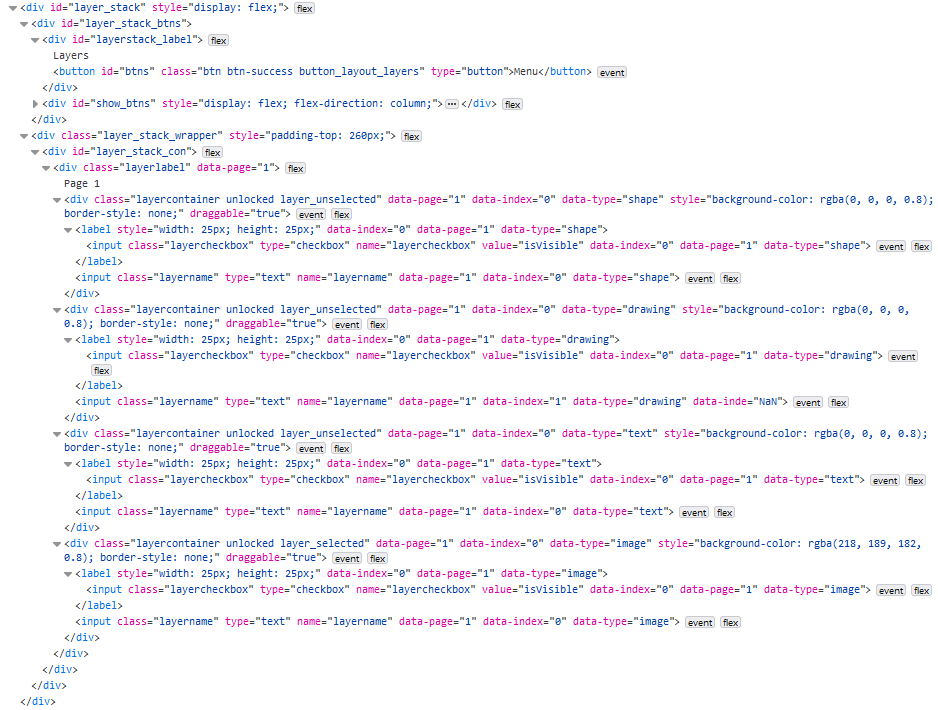
\includegraphics[width=1\textwidth]{"images/layer-stack.png"}
	\caption{Node-Tree Segment für den Aufbau der Layers}
	\label{fig:layer-stack}
\end{figure}

Während des Kopiervorgangs von Layers, der durch die Funktion dublicateLayerByElement hervorrufen wird, wird zunächst die Layer per cloneNode(true) dupliziert und erhält einen inkrementierten Index in seinen data-index Attributen. Das zugehörige duplizierte Element erlangt den gleichen Index. Die duplizierte Layer wird hinter der source Layer im layer\_stack eingefügt. Folglich liegt das kopierte Element auf dem source Element in der z-Achsenreihenfolge. Außerdem wird der kopierten Layer ein input event mit der hideLayer-Funktion und ein click event mit der markLayer-Funktion angeheftet. Zusätzlich wird erneut moveLayer auf dem layer\_stack\_con ausgeführt, damit die drag events auf der neuen Layer aktualisiert werden. Die Funktion dublicateElement kopiert das Element der duplizierten Layer. In diesem Prozess wird das Nodestrukturobjekt aus seiner Liste geholt und anhand dessen Vorlage ein neues Nodestrukturobjekt, samt Eigenschaftsobjekt, erzeugt. Dessen properties werden mit den Werten der source Objekte initialisiert. Bei kopierten drawingLayer-Objekten ist zu beachten, dass das Objekt mit der deepCopy-Funktion nicht nur die Referenzen kopiert, sondern tatsächlich das Objekt und alle Unterobjekte in paths. Das kopierte Objekt wird seiner Elementliste hinzugefügt und die source Layer bleibt ausgewählt, während die kopierte Layer abgewählt ist. Locked und kopierte Objekte behalten ihren locked-Status.

\subsection{Box Mode Modi}
Bei jeder Operation auf einem Element im Operations Bar und Tools, außer bei den Operationen zum Hinzufügen von Elementen, wird zunächst geprüft, ob der Editor im Box Mode oder Layer Mode arbeitet, und ob die Layer locked ist. Alle Operationen im Box Mode besitzen einen operationseigenen Modus. Jeder Modus wird mit seinem Boolean-Wert in einem Modi-Array protokolliert. Die Modusliste für Operationen auf Text heißt userModes, für Drawings userModesDrawer, für Shapes userModesGeometry und für Images userModesImages. Bei den meisten Buttons im Reader und Editor wird eine Funktion resetAllModes ausgeführt. Sie setzt alle Modilistenbestandteile auf false. Dadurch kann ein vorheriger Operationsmodus verlassen werden. Durch die Ausführung einer neuen Operation, wird ihr Modus aktiviert.

\subsection{Zoomfunktionalität}
Die Zoom-Operationen werden mit einer Verzögerung von 300 ms ausgeführt. Erfolgen Zoom-Operationen zu schnell hintereinander, wird ohne diese Verzögerung ein Fehler geworfen. Der Fehler warnt, dass nicht gleichzeitige Renderoperationen in derselben CANVAS ausgeführt werden können. Im Verlauf der Funktionen zoomIn, zoomOut und enterZoomFactor wird zunächst eine Funktion placeEditorElements aufgerufen, die die controlBoxes und Editorelemente passend zum Zoomfaktor auf der Seite platziert. ControlBoxes behalten beim Zoomen ihre Größe bei. Abschließend werden alle Seiten mit dem neuen Zoomfaktor gerendert.

\subsection{Downloadfunktion}
Die Downloadfunktion für Editorelemente wird in einer promise chain ausgeführt. Zunächst wird der aktuelle Zoomfaktor gespeichert und das PDF-Dokument wird auf 500 \% Prozent im Editor vergrößert. Das hat den Hintergrund, dass alle Editorelemente anschließend als DataURL in Form eines PNG-Bildes in das PDF mit originalPDFBytes eingebettet werden. Genauer gesagt werden alle editimgs mit der Klasse visible zu einem DataURL konvertiert. Editimgs erhalten die Klasse hidden, wenn Layers im Layers Seitenmenü über die grüne checkbox ausgeblendet wurden. Nach der Einbettung der PNG-Bilder mit 500 \% Skalierung wird die Datei zu einem ZIP-Archiv komprimiert. Das Archiv wird zu einem ObjectURL umgewandelt und durch ein neu erstelltes Anchor-HTML-Element, was dem Body hinzugefügt wird, gedownloaded. Anschließend wird das Anchror-Element wieder vom Body entfernt und das PDF wird auf die vorherige Skalierung zurückgezoomt. Im nächsten Abschnitt werde ich einige Tests der PDF Web App durchführen, um Funktion und Performance zu erörtern. 